\section{Technical Approach I --- Core Semantics}
\label{sec:core}

Five modifiers make a single component accessible --- labelling, roles, state, touch-target size, and
scalable type. They fix the most common and most damaging screen-reader defects.

\subsection{Content descriptions: naming visual elements}

A screen reader cannot see an icon; it can only read the icon's text alternative --- in Compose, the
\code{contentDescription} parameter. Three rules make a good label:

\begin{itemize}[leftmargin=1.4em]
	\item \textbf{Succinct \& action-oriented.} Avoid ``Image of'' / ``Button to''. The element's name is
	      announced separately.
	\item \textbf{Localized.} Always use \code{stringResource()} so labels translate with the device
	      language.
	\item \textbf{Hide the decorative.} Purely decorative graphics must be removed from the tree so
	      they do not add noise.
\end{itemize}

\begin{lstlisting}[caption={Meaningful icons get a localized label; decorative art is hidden.},captionpos=b]
// Meaningful control — announced as "Search podcasts, button"
Icon(
    imageVector = Icons.Filled.Search,
    contentDescription = stringResource(R.string.cd_search)
)

// Decorative cover tile — next to a text title, so it adds nothing for TalkBack
Box(
    modifier = Modifier.size(56.dp).background(color)
        .semantics { hideFromAccessibility() }   // Compose 1.8+; still visible to UI tests
)
\end{lstlisting}

In practice: Instagram labels its action buttons (``Like'', ``Comment'') but passes \code{null} to
the decorative story gradients, so screen-reader users jump straight between real content.

\subsection{Roles and state descriptions on custom controls}

Material components carry their own semantics, but a custom control built from a bare \code{Box} tells
assistive tech nothing. We must declare two things explicitly: a \textbf{role} (so TalkBack appends
``Button''/``Switch'') and, for anything toggleable, a \textbf{state description} (the dynamic
``Playing''/``Paused''). Our circular player button, taken directly from the app, does both:

\begin{lstlisting}[caption={\texttt{PlayToggle.kt} --- a custom control with an explicit role and a dynamic state.},captionpos=b]
@Composable
fun PlayToggle(isPlaying: Boolean, onToggle: () -> Unit) {
    val name = stringResource(if (isPlaying) R.string.cd_pause else R.string.cd_play)
    val state = stringResource(if (isPlaying) R.string.state_playing else R.string.state_paused)
    Box(
        modifier = Modifier.size(72.dp).clip(CircleShape).background(primary)
            .clickable(onClick = onToggle, role = Role.Button)
            .semantics {
                contentDescription = name       // "Play" / "Pause"
                stateDescription = state         // "Playing" / "Paused"
                role = Role.Button
            },
        contentAlignment = Alignment.Center
    ) {
        Icon(imageVector = icon, contentDescription = null) // handled by the Box
    }
}
\end{lstlisting}

TalkBack now announces \emph{``Pause, button, Playing''} --- name, role, and state --- which is
exactly how Spotify's custom playback control behaves.

\subsection{Touch-target sizing}

Users with motor impairments, or anyone tapping on a moving bus, need a target they can hit
reliably. Material Design mandates a minimum interactive size of \textbf{48\,dp $\times$ 48\,dp}
(WCAG~2.5.5 asks for 44\,px). The visual icon can stay small; only the \emph{touchable area} must
grow. Compose does this automatically for Material components and, for custom ones, via
\code{minimumInteractiveComponentSize()}:

\begin{lstlisting}[caption={A 24\,dp icon with a guaranteed 48\,dp touch target.},captionpos=b]
IconButton(
    onClick = onToggleBookmark,
    modifier = Modifier
        .minimumInteractiveComponentSize()   // expands hit area to 48dp, no visual change
        .clearAndSetSemantics {}             // (see advanced section)
) { Icon(Icons.Filled.BookmarkBorder, contentDescription = null) }
\end{lstlisting}

This is the same pattern Gmail uses for the small ``star'' icon: a 24\,dp glyph with a 48\,dp hit
area, so users do not open the email by accident when they meant to star it.

\subsection{Scalable typography}

Android~14 introduced \textbf{non-linear font scaling} up to 200\%: small text grows a lot while
already-large headings grow less, preserving hierarchy. To benefit, code must separate \emph{text
	size} from \emph{layout size}:

\begin{enumerate}[leftmargin=1.4em]
	\item Text sizes always in \code{sp} --- Compose applies the non-linear math automatically.
	\item Paddings and constraints always in \code{dp}.
	\item \textbf{Never} hard-code a \code{height()} on a text container; use \code{defaultMinSize} or
	      padding so it can grow.
\end{enumerate}

Figure~\ref{fig:fontscale} shows why the third rule matters: a fixed-height card clips its text at
200\%, while the \code{sp}-based card grows gracefully. Our \code{Type.kt} defines every style in
\code{sp}, so the app passes this test out of the box.

\begin{figure}[h]
	\centering
	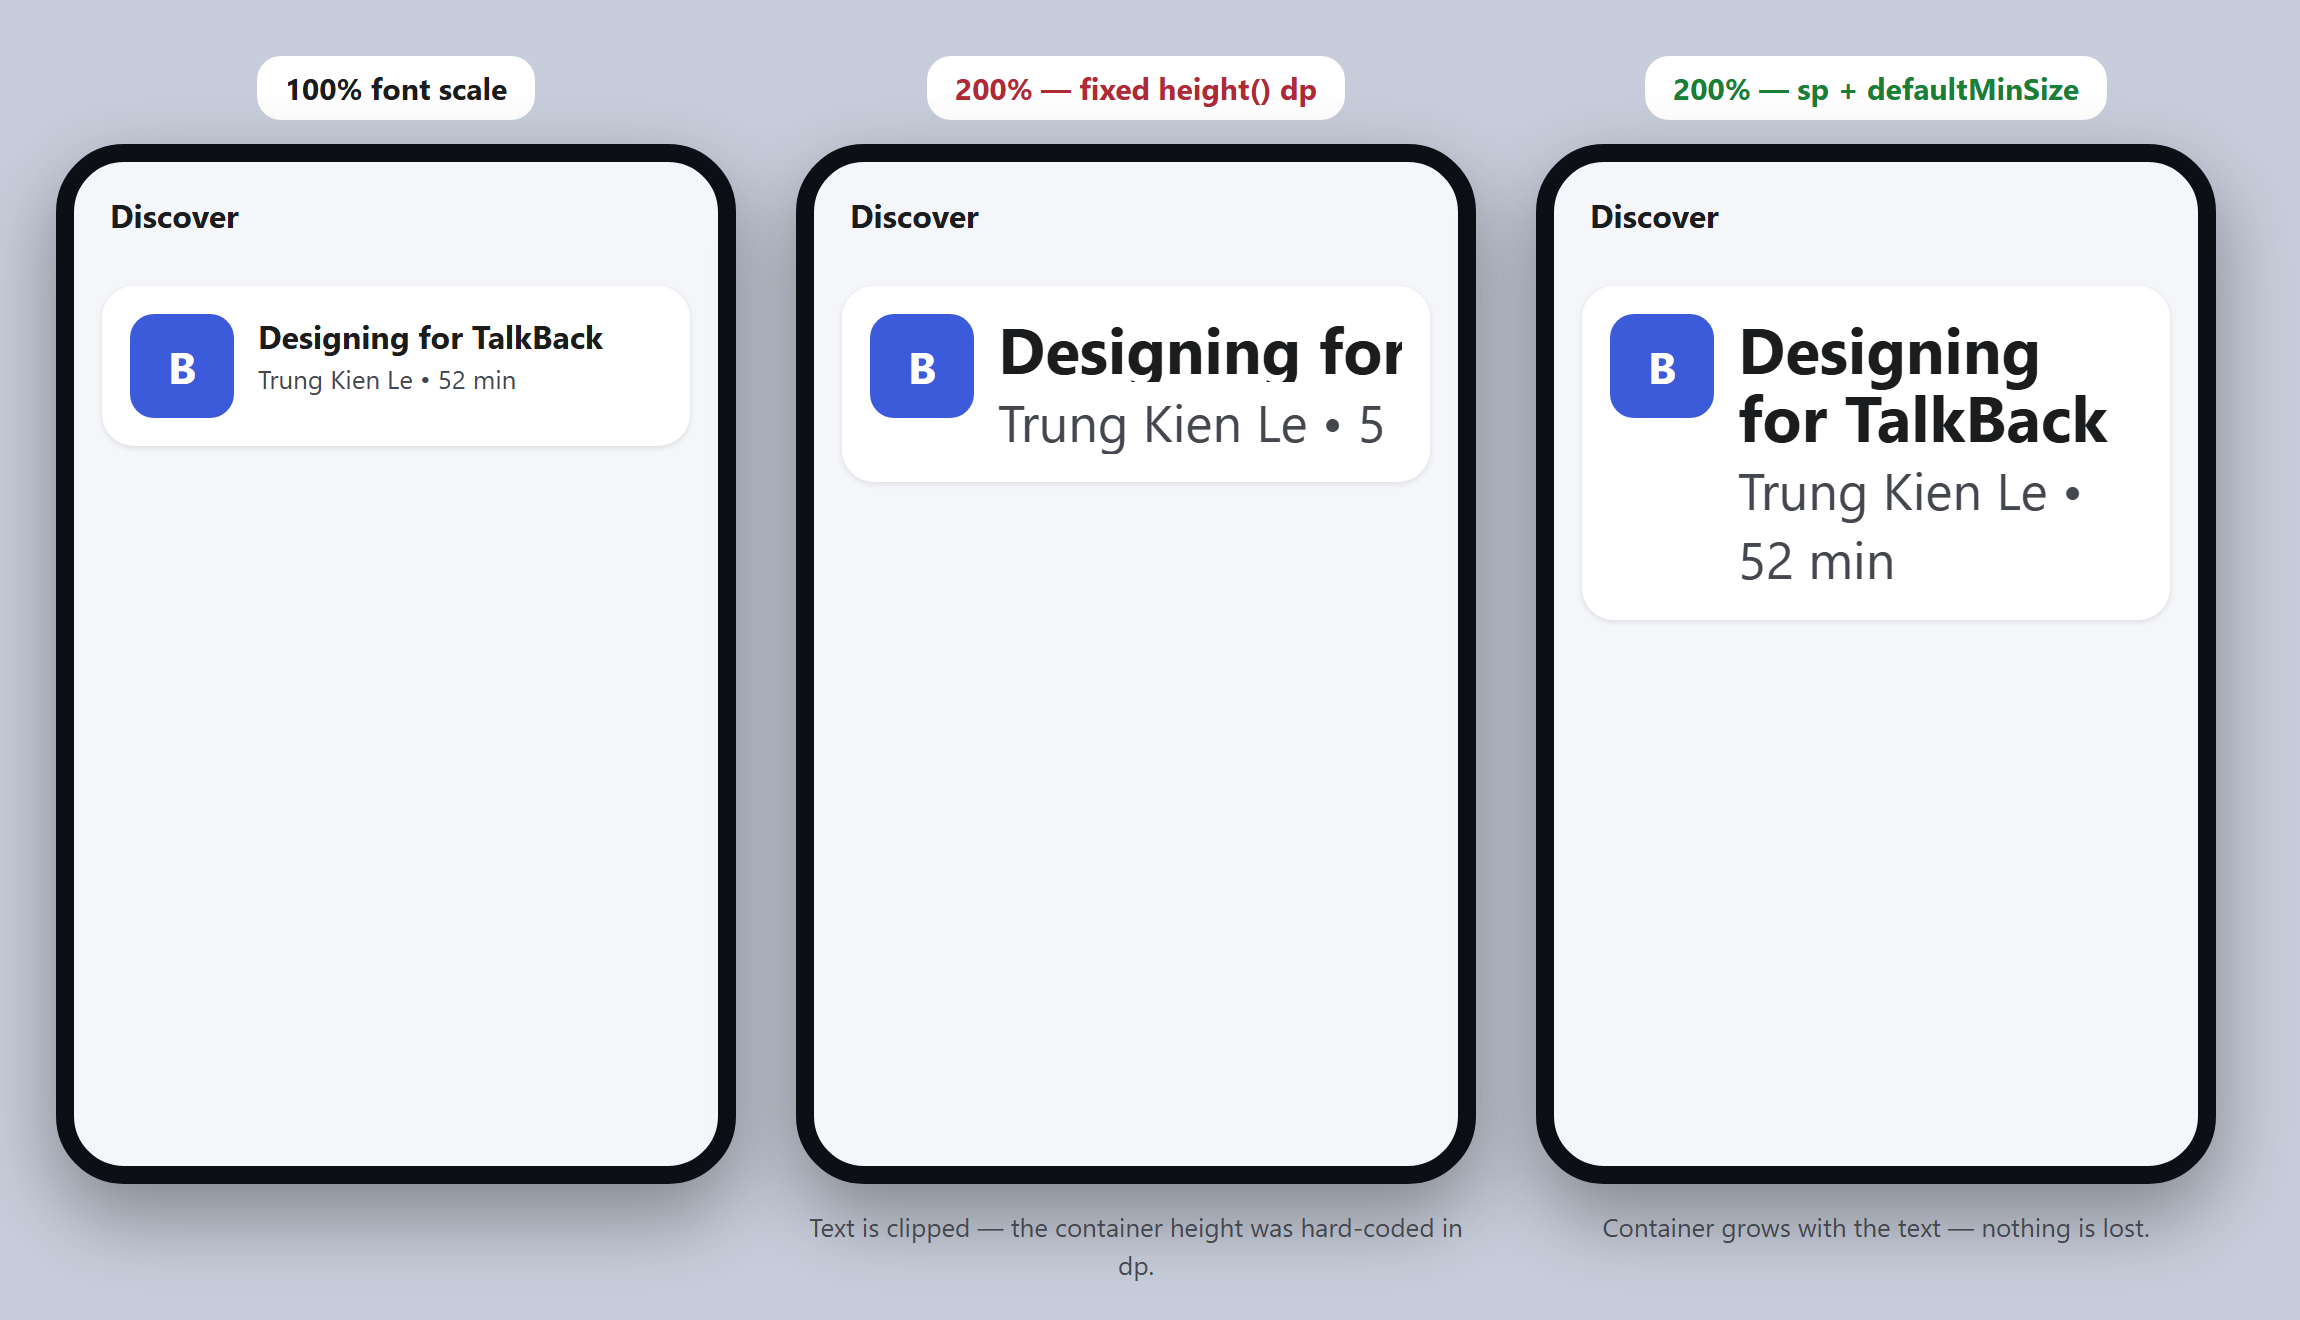
\includegraphics[width=\textwidth]{images/fontscale.png}
	\caption{The same card at 100\% and at 200\% font scale. A hard-coded \code{height()} in dp (centre)
		clips the title; \code{sp} text with \code{defaultMinSize} (right) lets the container expand so
		nothing is lost.}
	\label{fig:fontscale}
\end{figure}

\subsection{Heading navigation}

Finally, marking section titles with \code{semantics \{ heading() \}} lets TalkBack users jump
heading-to-heading instead of swiping through every item --- the screen-reader equivalent of
skimming. We apply it to the app-bar titles and the ``Fresh for you'' / ``Episodes'' headers.
